%!TEX root = ../template.tex
%%%%%%%%%%%%%%%%%%%%%%%%%%%%%%%%%%%%%%%%%%%%%%%%%%%%%%%%%%%%%%%%%%%
%% background_relatedwork.tex
%%
%% Chapter with Background and Related Work
%%
%% REVIEWED by Diogo Gato 2022/03/28
%%%%%%%%%%%%%%%%%%%%%%%%%%%%%%%%%%%%%%%%%%%%%%%%%%%%%%%%%%%%%%%%%%%

%REVIEWED 2022/04/15
% W/CORRECTIONS FROM PROF 30/03/2022

\typeout{NT FILE background.tex}

\chapter{Background}
\label{cha:background}


\section{Introduction} 
\label{sub:if_you_use_this_template} 

In this chapter we will provide to the reader the necessary background. We will start by introducing the system in which our thesis work will be implemented and that provide us the data that will be used. Then, we will advance to a theoretical introduction to our main analysis theme, the wind turbines, providing a first introduction to its context in nowadays, how their downtimes are classified and their major components. We will finish this chapter by introducing the area that we will use to accomplish our goal, machine learning.

\section{CGI RMS - Renewable Monitoring System} 
\label{sub:if_you_use_this_template} 

CGI Renewable Monitoring System (\acrshort{rms}) is a system that “comprises an integrated set of tools to maximize energy production, increase availability, control energy losses, and improve overall operational performance with direct impact on business revenues".

Its scope includes all the 3 major renewable energies: wind, solar and hydro. In 2019, it had multiple clients with a total combined portfolio of over 8,000 generators, and approximately 15 GW installed capacity distributed over 3 continents: North America (with 5,495 MW) South America (with 1,261 MW) and Europe (with 8,089 MW) \cite{OLD_8}. It has 4 major modules \cite{OLD_8}:

\begin{enumerate}
\item
Monitor: with a screen with possible dashboards and tools with real time data, allows to assist both managers and field teams in acquire all the necessary information to manage their assets.

\item
Analyze: provides a global overview of portfolio performance by providing trend analysis, benchmark indicators and key operational dashboards and reports.

\item
Predict: by using machine-learning algorithms and continuous monitoring of real-time data, allows to anticipate potential failures. It allows also to build digital twins and use them as a baseline for behavior comparison.

\item
Operate: this module is designed for control rooms. It provides multi-screen with a clear real-time overview of all assets and a step-by-step workflow to guide operators, remote control, and intelligent alarm management.
\end{enumerate}

CGI \acrshort{rms} stands-out by providing real-time portfolio supervision (represented in Figure 2.1 by the monitoring dashboard) and control, automatic generation and sharing of reports and data exports, key performance indicators calculated and updated according to the real-time data, long-term storage of historical data for performance analysis and tools to analyze the data (like the Data Analysis tool, represented in Figure 2.2) and performance of their assets according to what it should be expected with dashboards like the power curve analysis, among other features.

\begin{figure}[htbp]
	\centering
	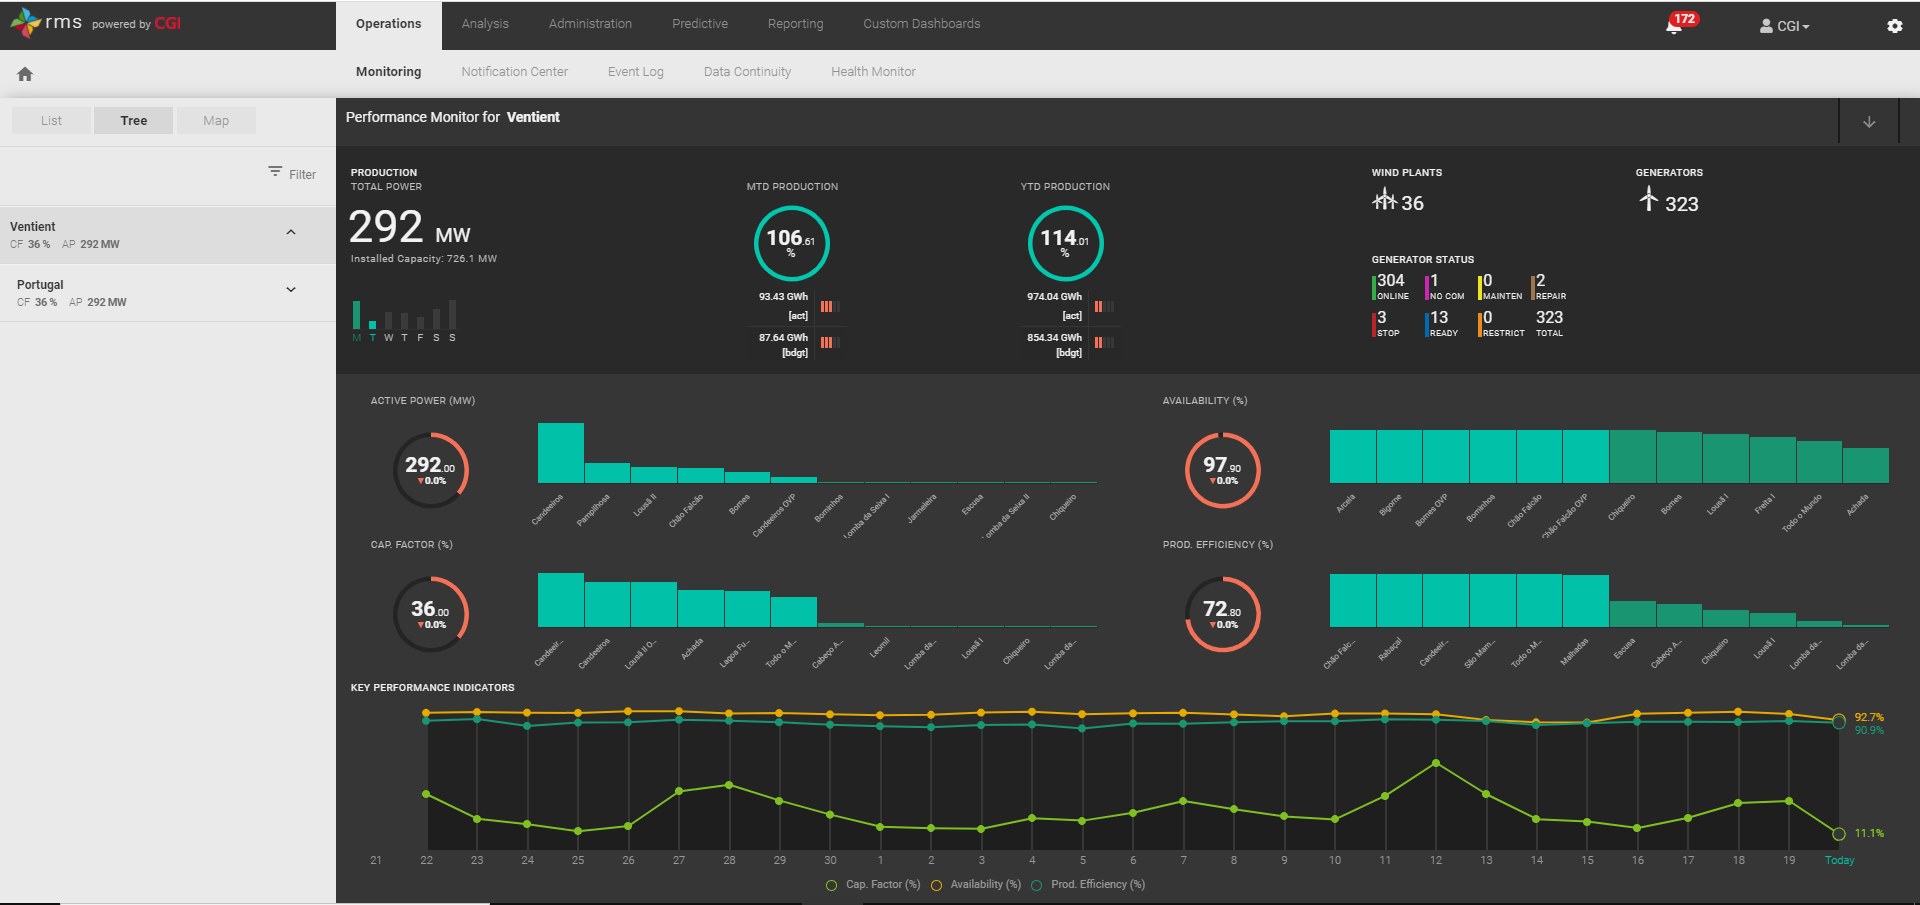
\includegraphics[width=\textwidth]{Chapters/Figures/background_fig2.PNG}
	\caption{Dashboard of general monitoring. The user can have an overview of the state, performance and notifications and alarms that exist on their parks and assets.Source: \cite{CGIRMS} }
	\label{fig:Figuras_Tree_silhouettes-vectorial}
\end{figure}


\begin{figure}[htbp]
	\centering
	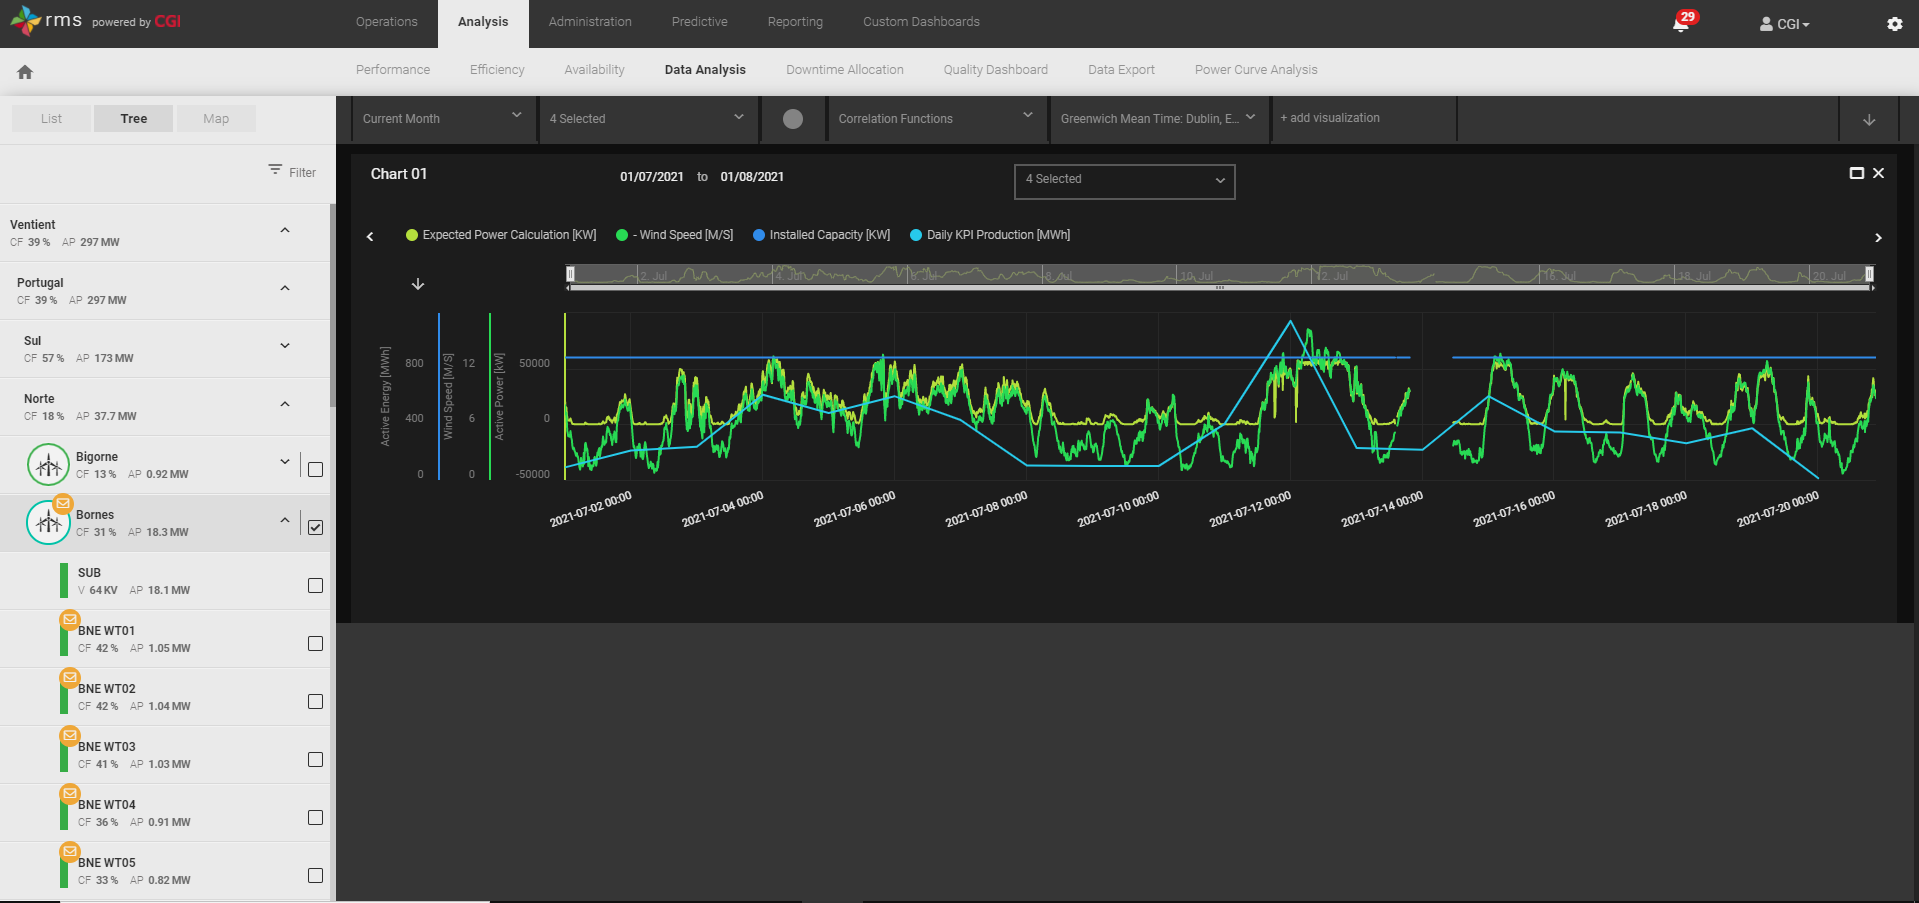
\includegraphics[width=\textwidth]{Chapters/Figures/background_fig3.PNG}
	\caption{CGI RMS Data Analysis tool. It allows to select certain variables, key performance indicators and signals and compare their values in a certain time interval. It also allows to apply a correlation function on those variables. Source: \cite{CGIRMS} }
	\label{fig:Figuras_Tree_silhouettes-vectorial}
\end{figure}


\section{Wind Turbines} 
\label{sub:if_you_use_this_template} 

Our study will focus into one of the major renewable energy technologies: wind turbines. This renewable energy source is increasingly year by year. As we can see in Figure 2.3, in 2019 in the whole World combined, there was a growth of 12,14\% in terms of wind energy generation. In Portugal only, these numbers are similar, with a total growth of 8,48\% in terms of wind energy produced, compared to the previous year. According to the latest date of IRENA (International Renewable Energy Agency), the global investment in renewable energy technologies is 46,56\% in wind energy \cite{OLD_33_GENERAL}.

The data available in terms of the grow in these two renewable energy sources, are major factors that motivate the development and improvement of technologies like the CGI \acrshort{rms} and studies like the one that was developed in this Master Thesis.


\begin{figure}[htbp]
	\centering
	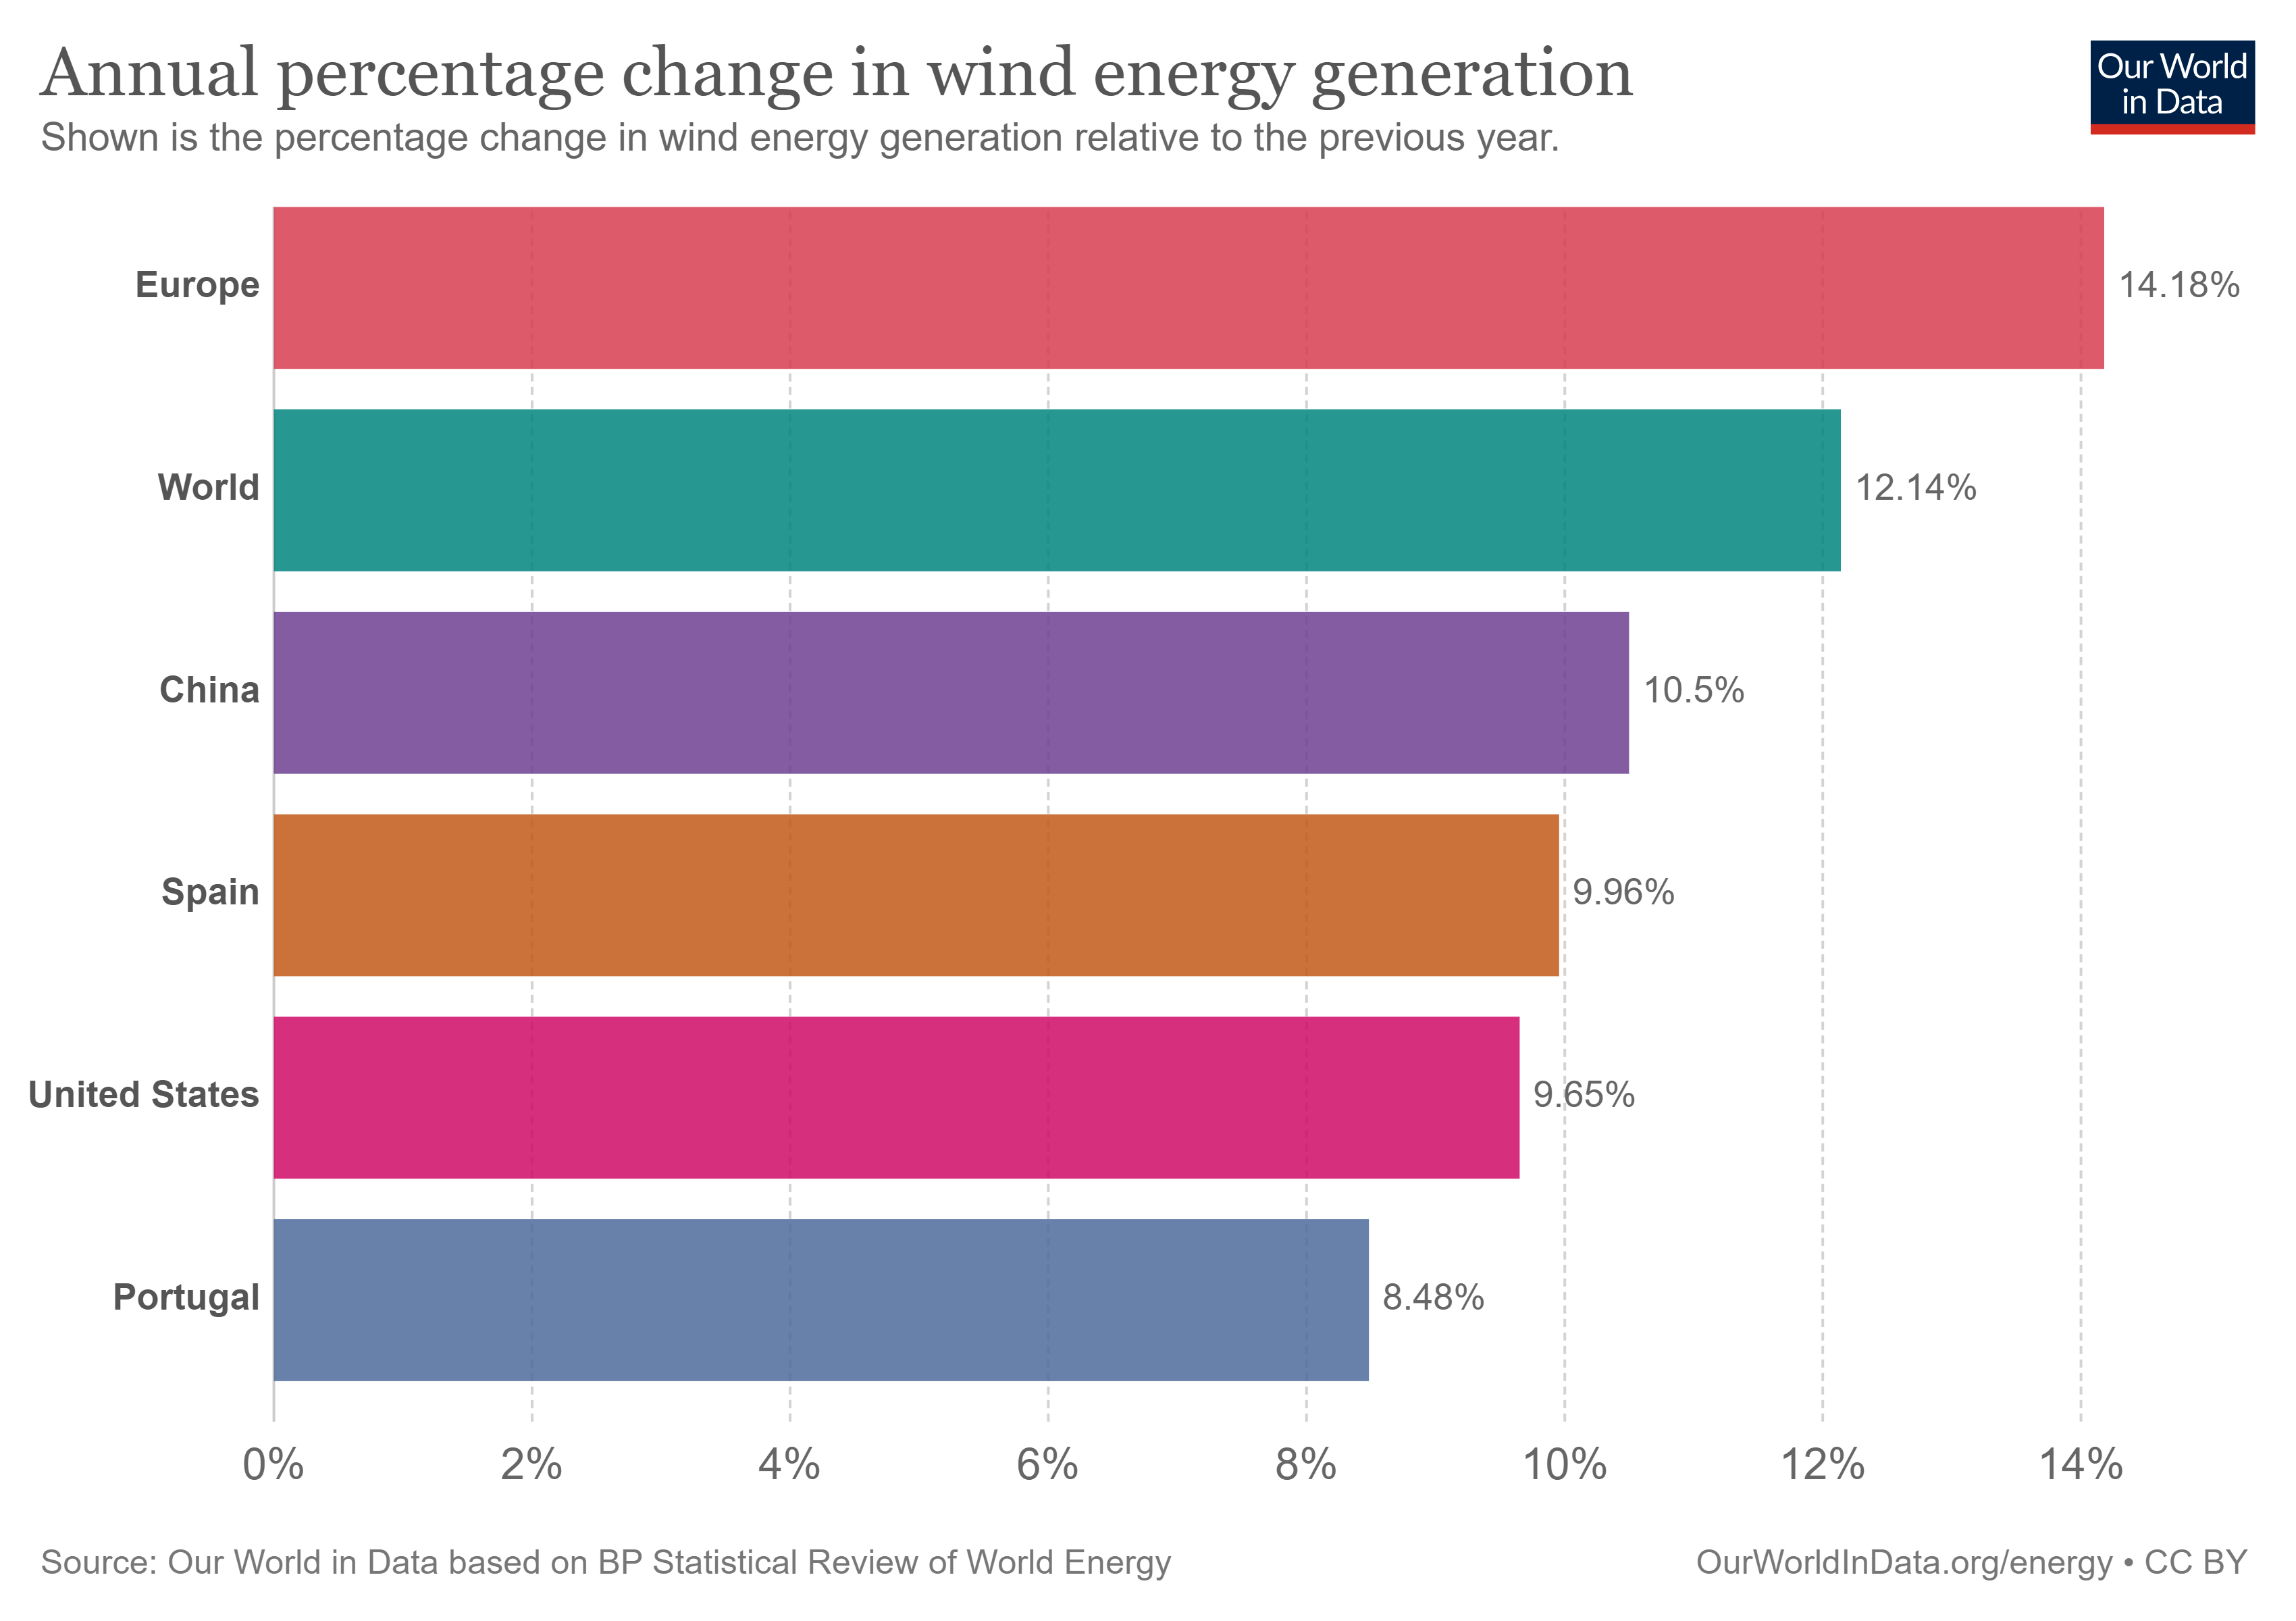
\includegraphics[width=\textwidth]{Chapters/Figures/background_fig4.PNG}
	\caption{Shown is the percentage change in wind energy generation relative to the previous year, according to OurWordInData. \cite{OLD_33_GENERAL} }
	\label{fig:Figuras_Tree_silhouettes-vectorial}
\end{figure}


In this chapter, we are going to introduce the basics of each of the wind turbines that allow the reader to acquire a general knowledge of them and some key concepts that will provide the basics to understand this Master Thesis goals. We will start by introducing how a wind park is composed, presenting the major components of each of their asset and finalizing with the factors (internal or external) that may cause failures in these same assets.


The wind brings kinetic energy associated with it. This energy, when passes through the wind turbine, rotate the blades and consequently the rotor. With this, the kinetic energy is transformed into mechanical energy that can acquired and transformed into electric energy and supplied to the grid \cite{OLD_29_WIND} \cite{OLD_31}.
Wind turbines may be classified as two major types: horizontal-axis turbines and vertical-axis turbines, represented in Figure 2.4 in the left and right images, respectively. The more common are the horizontal-axis turbines, that are also composed with gearboxes to accelerate the slow rotation of the blades, to make it strong enough for the generator. The length of the blades is the biggest factor that determines the amount of energy that a wind turbine can generate.

\begin{figure}[]
	\centering
	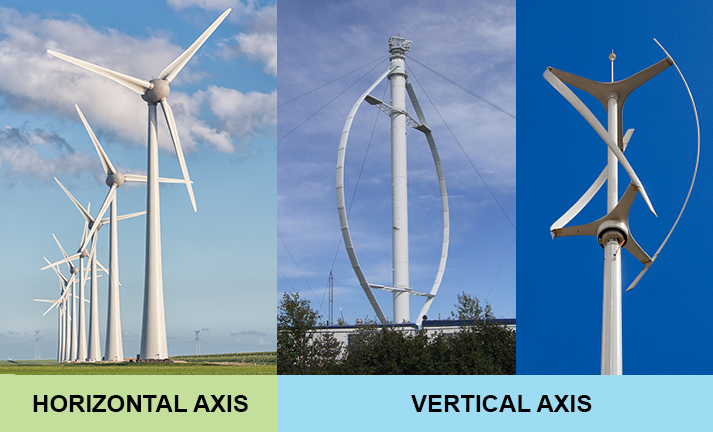
\includegraphics[width=\textwidth]{Chapters/Figures/background_fig5.png}
	\caption{Different types of Wind Turbines: horizontal (left) and vertical (right) Source: Kid's Korner (apogee.net) }
	\label{fig:Figuras_Tree_silhouettes-vectorial}
\end{figure}


%%%TODO: Adicionar mais ou menos enquanto varia a Installed Capacity de uma turbina

A wind power plant, also known as wind farm, is the combination of multiple turbines. A wind park may have hundreds of wind turbines, like the Capricon Ridge Wind Farm, in Texas, United States, that have more than 400 wind turbines making it a park with an installed capacity of 662,5 MW \cite{OLD_35_WIND}.
As we can see in the charts of Figure 2.5 in terms of wind energy sources, in 2019, the electricity generated per year in the World was 1.416,95 TWh and 13,69 TWh in Portugal. The total installed power worldwide was 622,25 GW and in Portugal was 5,22 GW \cite{OLD_33_GENERAL}.


\begin{figure}[htbp]
	\centering
	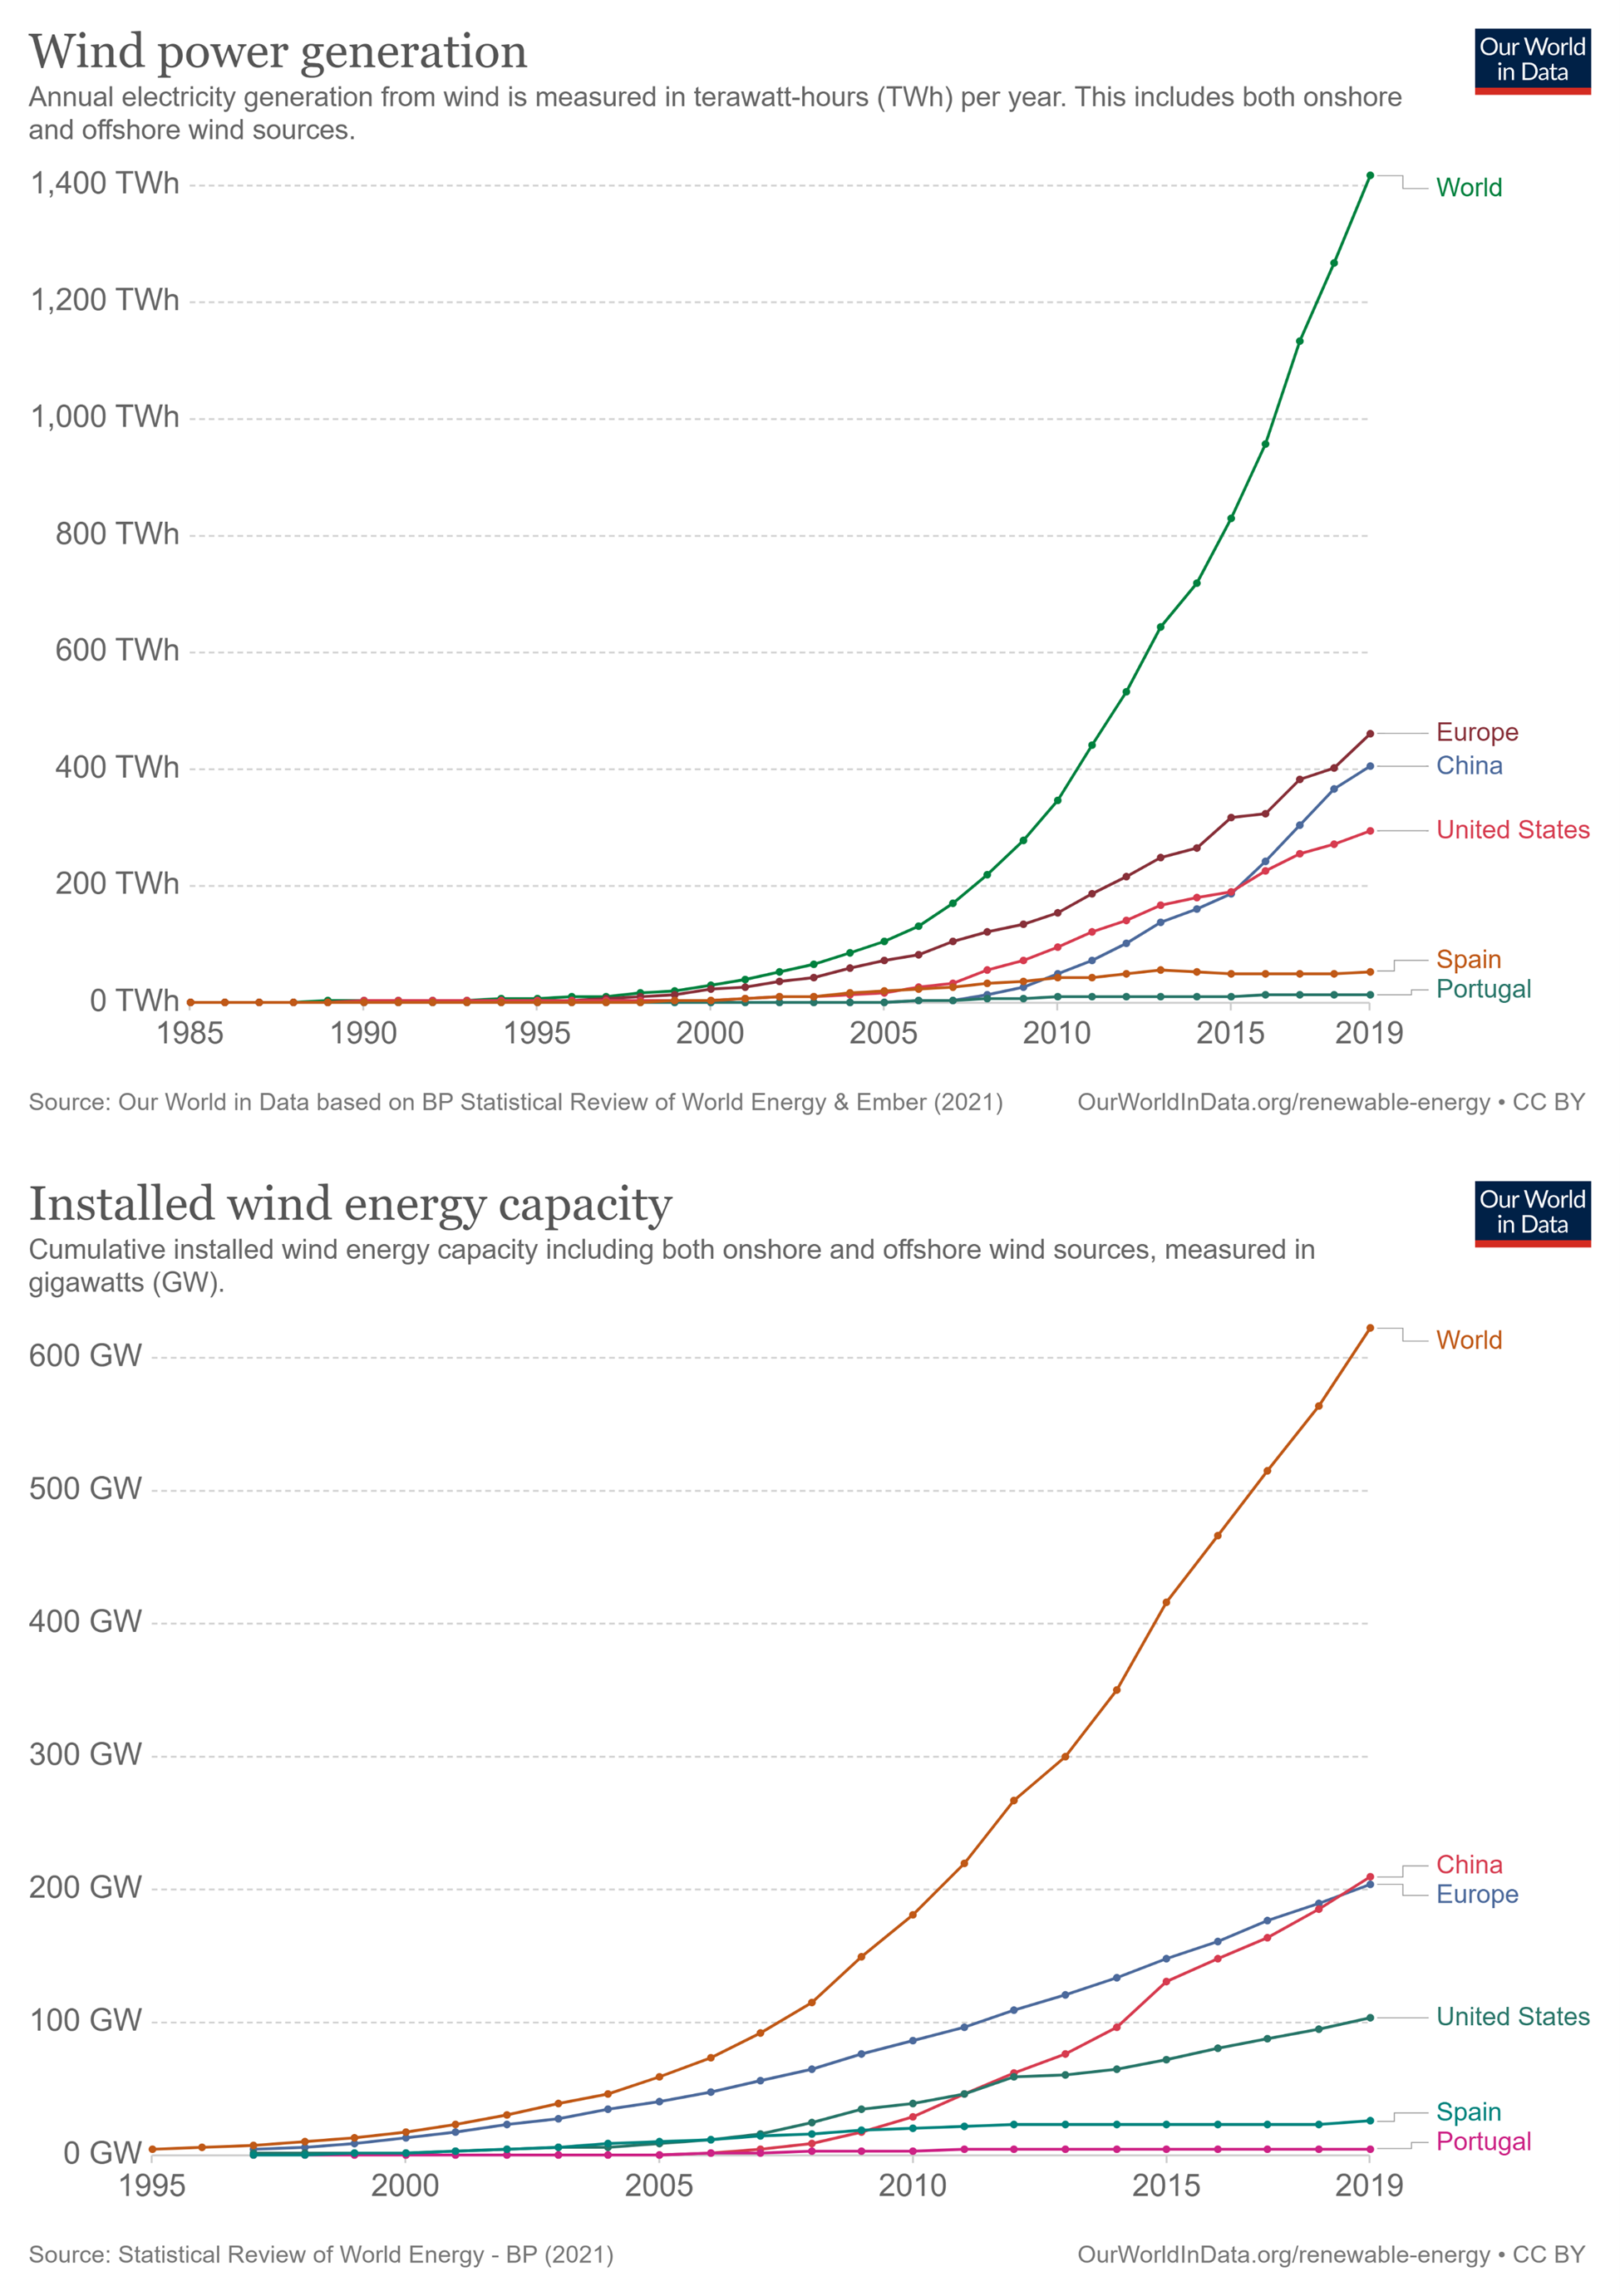
\includegraphics[width=\textwidth]{Chapters/Figures/background_fig6.PNG}
	\caption{Electricity generated from wind energy sources (up image) and  installed wind capacity (down image) in 2019 in two continents (World, Europe) and four countries (China, United States, Spain and Portugal). \cite{OLD_33_GENERAL} }
	\label{fig:Figuras_Tree_silhouettes-vectorial}
\end{figure}

%TODO: Format the Paragraphs and respective images

\subsection{Downtime Classification} 
\label{sub:if_you_use_this_template} 

Faults in a wind turbine, causes unscheduled maintenance and consequently, loss in the production of energy. A wind turbine has many and complex components that, without the required maintenance and a predictive system of their conditions, may cause the wind turbine to stop working and, may cause the total failure on a component that may cause costs in terms of their replacement, as well as downtime on a wind turbine, which leads to a drop in production.
Downtimes in a wind power plant are classified in two major categories, like in the wind power plant:
 
 %The figure 2.6 presented below, shows the Downtime Allocation Tree available in CGI RMS and that distributes the major failures that may occur in a wind farm

\begin{enumerate}
    \item{Internal Causes:}
These internal downtimes can be caused by wind turbine direct failures or internal \gls{BoP} failures. These failures are registered also as planned, unplanned or caused by civil or electrical repairs, with each of these being classified in a lower level of the specific cause of the failure, like wind turbine maintenance, failures, among others.

    \item{External Causes:}
The external factors that may cause downtime to a wind power plant are grouped as external to the wind turbine, external \gls{BoP} failures or curtailment downtimes. The specificities of these failures may be caused by environment conditions, exclusion causes, operations on the grid, among many others.
\end{enumerate}

The failures that we are going to predict in this thesis are the ones concerning internal causes downtimes.

%\begin{figure}[htbp]
%	\centering
%	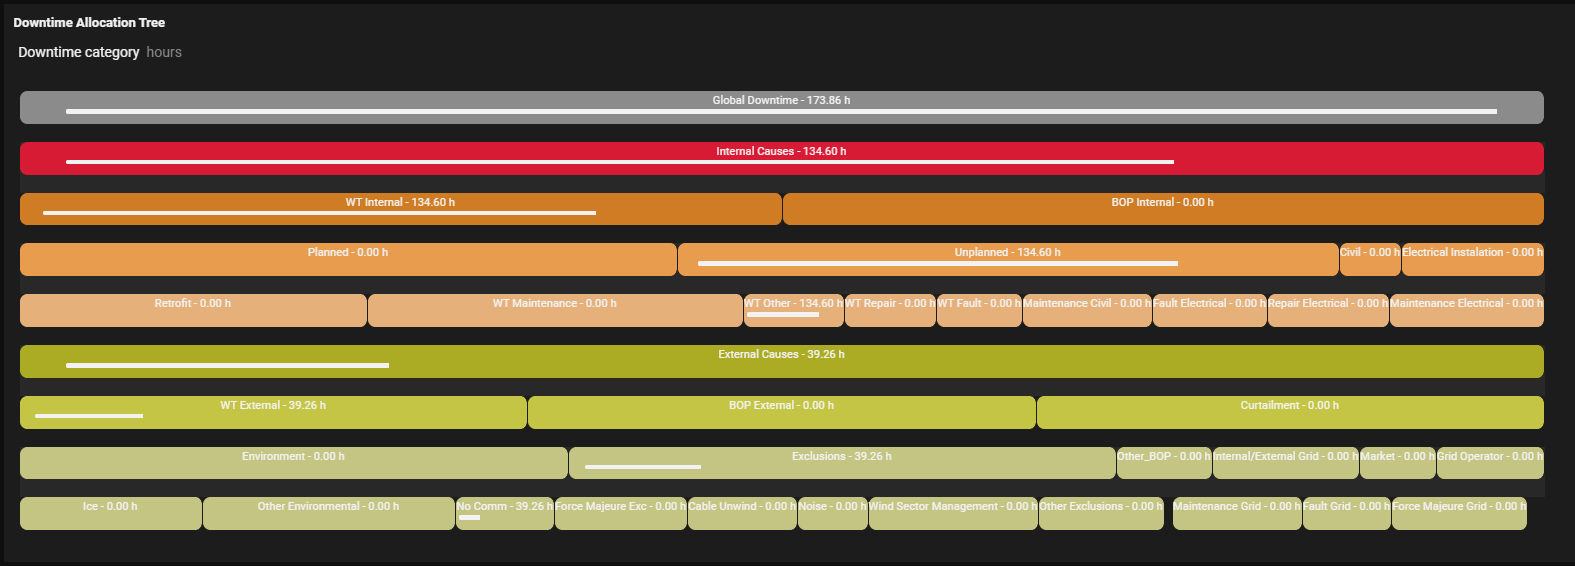
\includegraphics[angle=-90,height=0.1]{Chapters/Figures/background_fig7.PNG}
%	\caption{Wind Downtime Allocation Tree. From the Global Downtime (gray) to the two major causes classification: internal causes (dark red) and external %(darker green). The data used to build this chart is from historical data that comes from signals from the wind park.}
%	\label{fig:Figuras_Tree_silhouettes-vectorial}
%\end{figure}


\subsection{Major Components} 
\label{sub:if_you_use_this_template} 

The wind turbine and its blades form the base component that capture the wind, in order to, and with the help of other components, transform it into electric energy supplied to the grid. In Figure 8, we present an example of some of the main components that compose a wind turbine.

The wind cause lift and rotation of the blades. With this, the rotor [ Figure 2.6 - 1], that is composed together by the blades and hub, starts to spin. Since, most of the times, the wind Itself does not make the rotor spin enough to produce energy, the gearbox rotor [ Figure 2.6 - 3] that “connects the low-speed shaft to the high-speed shaft and increases the rotational speeds from around 30-60 rotations per minute (rpm), to about 1.000-1.800 rpm [ Figure 2.6 - 2 and 4, respectively]. This is the rotational speed required by most generators [ Figure 2.6 - 5] to produce electricity”. To maintain the performance and guarantee that the high speed intensity may cause some failures and damages in the wind turbine, the anemometer and controller [ Figure 2.6 - 6] together, allows to control the machine according to the wind speed: “Starts up the machine at wind speeds of about 12 to 25 kilometers per hour (km/h) and shuts off the machine at about 88 km/h. Turbines do not operate at wind speeds above about 88 km/h because they may be damaged by the high winds.” \cite{OLD_29_WIND}. These components and others, that have a more secondary role, form the nacelle [ Figure 2.6 - 7].

The high complexity and cost of the gearbox, makes this system part one that is trying to be improved: if electricity can be produced by lower rotational speeds, then the necessity of gearbox disappears and, consequently, the price of a wind turbine drops and the faults that are caused by problems of this component also disappear.
The major component that makes part of the wind turbine tower is the yaw [ Figure 2.6 - 8] (composed by the yaw drive and yaw motor): this component, in the overall, “orients upwind turbines to keep them facing the wind when the direction changes” \cite{OLD_29_WIND}.


\begin{figure}[htbp]
	\centering
	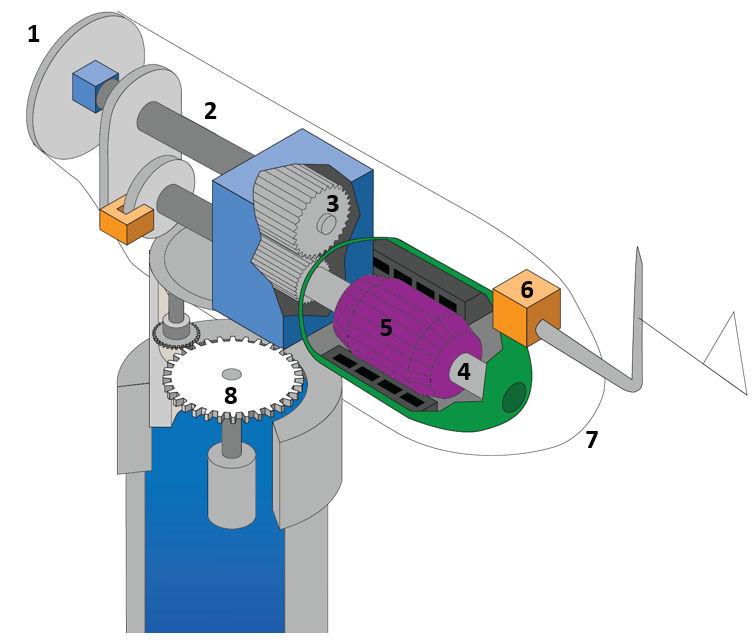
\includegraphics[scale=0.5]{Chapters/Figures/background_fig8.PNG}
	\caption{Wind turbine main components. [1] Rotor, [2] Low-Speed Shaft, [3] Gearbox, [4] High-Speed Shaft, [5] Generator, [6] Controller], [7] Nacelle, [8] Yaw (with Yaw Drive above and Yaw Motor below. Source: \cite{OLD_29_WIND} }
	\label{fig:Figuras_Tree_silhouettes-vectorial}
\end{figure}


\section{Machine Learning} 
\label{sub:if_you_use_this_template} 

%Machine Learning is the process of building a model that turns %information into knowledge. 
"Machine learning is the science of building systems that improve with data"\cite{FCT_AA}. By providing data into a machine learning, the model can analyze it and discover patterns that are useful for understanding relationships in data. This model must pass through a learning process so that it can improve its accuracy and reliability in providing correct outputs \cite{OLD_15_WIND} \cite{46_ML}.

The taxonomy of ML models is divided into two major types, as represented in Figure 2.7. In each taxonomy we also present the most common algorithms that are used. Some of these algorithms are going to be used in this thesis work.

\begin{enumerate}
    \item{Supervised Learning}
The main goal is to predict an output variable using labeled data as input. One important goal of these models is their adaptation to new input. To do that, we don’t want our model to be overfit, meaning, too much adapted to our training data. We always want our model to be as general as possible, so that the “supervised model defines the real ‘general’ underlying relationship”. A supervised learning algorithm may be a regression model, that predicts a numeric variable or a classification model, that it should classify the inputs into a set of classes.

    \item{Unsupervised Learning}
These models work only with input data, not having an output labelled data to compare. The main goal is to provide complex patterns that are hidden within data without any labels. The more used type of unsupervised learning is clustering. Clustering is the task of dividing the sample into a number of groups in which the data points from the same groups are similar to each other and dissimilar to the data points in other groups.
\end{enumerate}

ML also have two less used types and that are also more complex to implement: semi-supervised learning, that as the name indicates, it is a mix between supervised and unsupervised learning. It is used for cases that we mix a small amount of labelled data with a much larger unlabeled dataset; reinforcement learning, that is implemented as Pavlov’s dog study: occasional positive and negative feedback teaches the model to takes better decision in the next actions, meaning, in the next predictions \cite{46_ML}.

\begin{figure}[htbp]
	\centering
	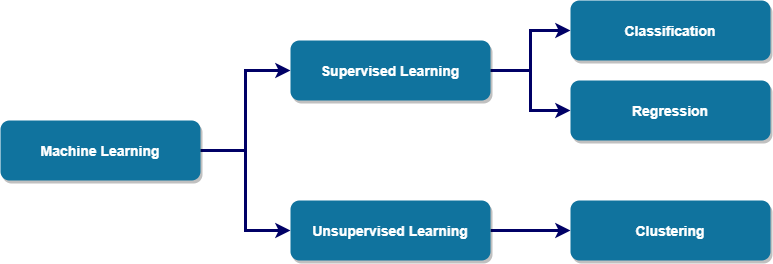
\includegraphics[width=\textwidth]{Chapters/Figures/background_fig9.PNG}
	\caption{Machine Learning taxonomy of the main types. Source: \cite{FCT_AA} }
	\label{fig:Figuras_Tree_silhouettes-vectorial}
\end{figure}


There exist 3 basics terms that we should know to understand ML \cite{46_ML}:
\begin{enumerate}
    \item{Dataset:}
The set of data that it is provided to train the model.
    \item{Features:}
"Important pieces of data that help us understand a problem. These are fed in to a Machine Learning algorithm to help it learn."
    \item{Model:}
It is the representation of what the ML algorithm has learnt during the training process from the data set and the features provided.
\end{enumerate}

The machine learning methodology follows 5 major steps: data collection and pre-processing; feature selection and extraction; model selection; validation; fitting the model \cite{OLD_15_WIND} \cite{46_ML}.

Another subfield of machine learning is deep learning. Deep learning is based in a layered structure of algorithms called artificial neural network that makes intelligent decisions on its own. One important detail of these types of algorithms is that they need a large amount of data to become more efficient that the typical supervised algorithms. The larger the dataset, better the algorithm will surpass the traditional machine learning algorithms \cite{ML_Deep_Learning_2} \cite{ML_Deep_Learning}.


\section{Conclusion} 
\label{sub:if_you_use_this_template} 

In this chapter we could understand how CGI \acrshort{rms} works, their main tools and its portfolio. It was also presented all the basic terms and operation of a wind turbine, how downtimes are divided, which is a basis of the classification of the failures that we are going to study and how the key components work together in a wind turbine, allowing us to understand the complexity of a wind turbine, from the nacelle to the yaw, and the importance of monitoring and predicting a failure in a component, so that all the other components that are connected don't be affected and consequently damaged, and the energy production can carry on without losses due to downtimes. It was introduced the machine learning area that will be used to implement anomaly detection models. Considering all the machine learning types, we can understand that the machine learning algorithms that should be used are the classification ones because our goal is exactly to understand in which cases, we are going to have a failure, or set of failures, and when we will have a normal operation time, for which we have labelled data.
